%!TEX root = ../fbi.tex

\section{Correlation functions}

We use the the cylindrical geometry of Figure \ref{fig:PEPS} to compute correlation functions for this wavefunction. By looking at how the correlation length changes with cylinder width $L$, we conclude that indeed all correlations are exponentially decaying in the 2D limit of large $L$. 

\begin{itemize}
\item Show correlation bounds for soft-core and hard-core states, correlation function fits.

\begin{figure}[H]
	\centering
	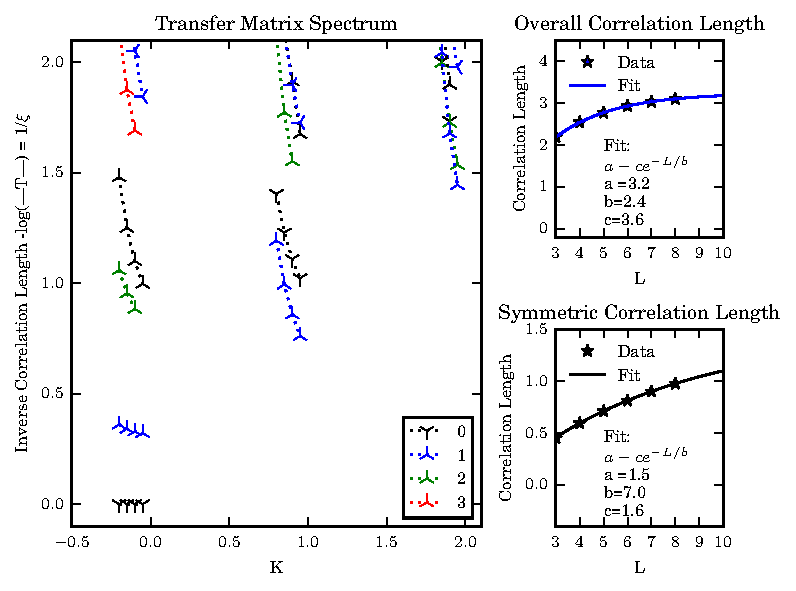
\includegraphics[width=\columnwidth]{TransferMatrixSpectrum_big.pdf}
	\caption{Placeholder for plots showing correlation bounds.}
	\label{fig:TMS}
\end{figure}

\item Emphasize that $\xi < L$ for the attainable system sizes $L$, so that we can have some trust in our results.
\item Show that correlations are isotropic.

\begin{figure}[H]
	\centering
	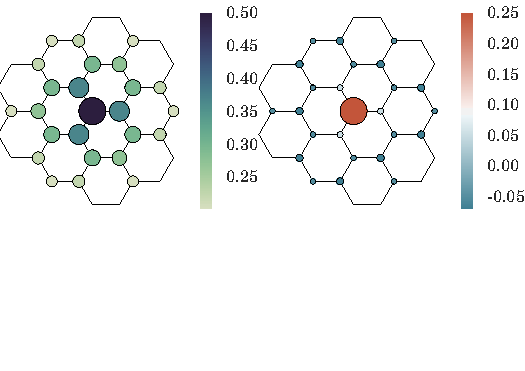
\includegraphics[width=0.6\columnwidth]{ShortDistanceCorrelations.pdf}
	\caption{Placeholder for 2D short distance correlation plot.}
	\label{fig:ShortCorr}
\end{figure}

\item Show that everything agrees with MC results, as far as those are available.
\end{itemize}


